\chapter{Instalação}

\section{MS-Windows}

Para instalar o InVesalius no MS-Windows, basta executar o programa instalador.
Quando aparecer uma janela pedindo para confirmar a execução do arquivo, clique
em \textbf{Sim}.

\begin{figure}[!htb]
\centering
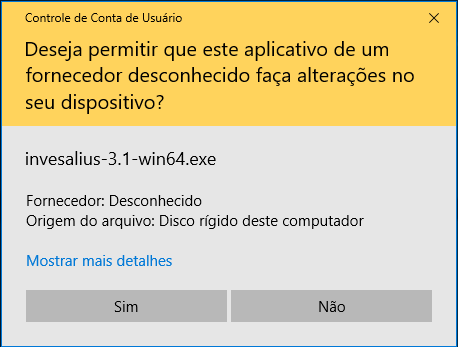
\includegraphics[scale=0.5]{installation_exec_pt.png}
\end{figure}

\newpage
Uma nova janela pedirá para selecionar o idioma do instalador. Selecione
o idioma e clique em \textbf{OK}.

\begin{figure}[!htb]
\centering
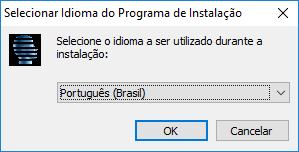
\includegraphics[scale=0.7]{installation_select_language_pt.png}
\end{figure}
 
\hspace{.2cm}

Em seguida, será exibida a janela do instalador. Clique em \textbf{Avançar}.

\begin{figure}[!htb]
\centering
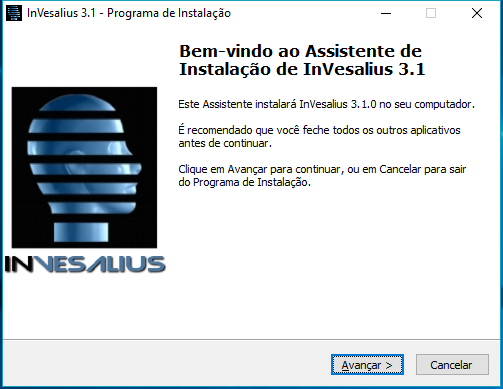
\includegraphics[scale=0.7]{installation_welcome_pt.png}
\end{figure}

\newpage

Selecione \textbf{Eu aceito os termos do Contrato} e clique em \textbf{Avançar}.

\begin{figure}[!htb] 
\centering
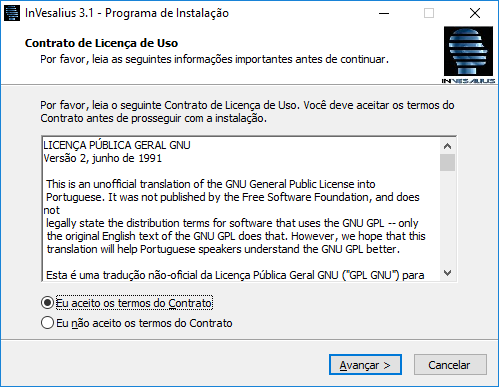
\includegraphics[scale=0.7]{installation_license_pt.png}
\end{figure}

\hspace{.2cm}

Clique em \textbf{Avançar} novamente. 

\begin{figure}[!htb]  
\centering
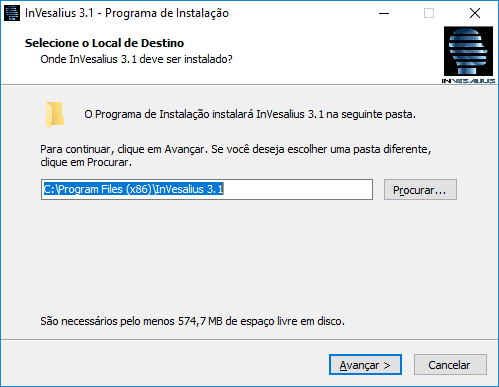
\includegraphics[scale=0.7]{installation_folder_pt.png}
\end{figure}

\newpage

Clique em \textbf{Avançar}.
\begin{figure}[!htb]
\centering
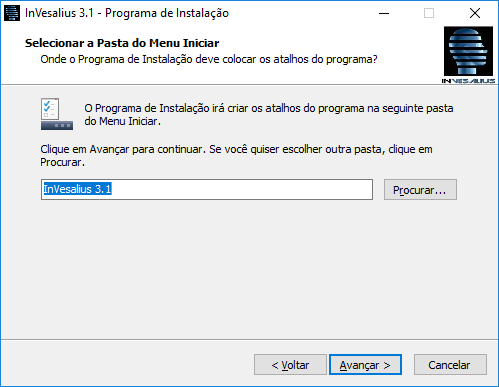
\includegraphics[scale=0.7]{installation_program_name_pt.png}
\end{figure}

\hspace{.2cm}

Selecione \textbf{Criar um ícone na Área de Trabalho} e clique em \textbf{Avançar}.

\begin{figure}[!htb]
\centering
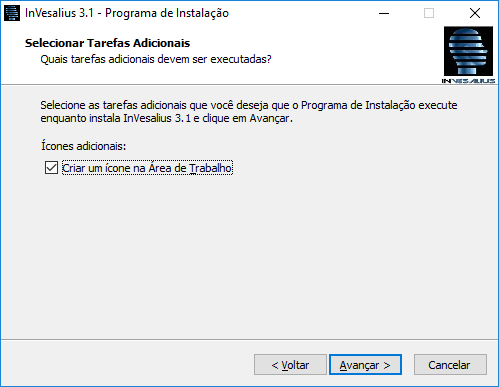
\includegraphics[scale=0.7]{installation_desktop_shortcut_pt.png}
\end{figure}

\newpage

Clique em \textbf{Instalar}.

\begin{figure}[!htb]
\centering
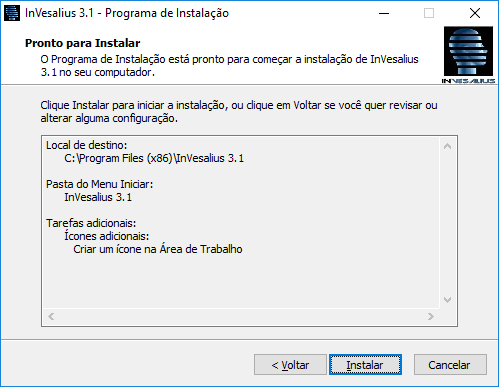
\includegraphics[scale=0.7]{installation_resume_pt.png}
\end{figure}

\hspace{.2cm}

Enquanto o software é instalado, será exibida uma janela com o progresso
da instalação.

\begin{figure}[!htb]
\centering
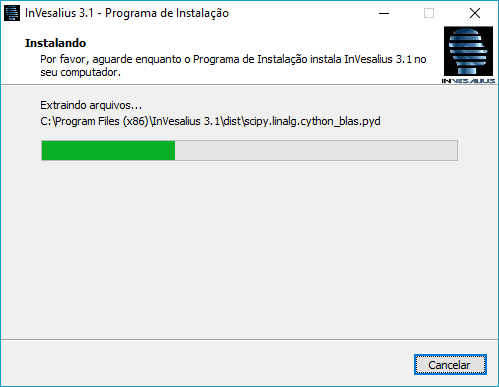
\includegraphics[scale=0.7]{installation_progress_pt.png}
\end{figure}

\newpage

Para executar o InVesalius após a instalação, clique em \textbf{Concluir}.

\begin{figure}[!htb]
\centering
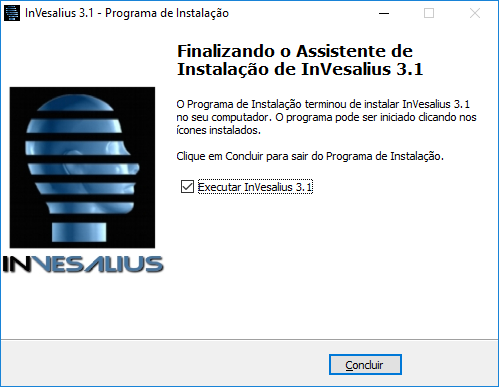
\includegraphics[scale=0.7]{installation_finish_pt.png}
\end{figure}

\hspace{.2cm}

Caso seja a primeira vez em que o software é instalado, será exibida uma janela
para selecionar o idioma do InVesalius. Selecione o idioma desejado e clique em
\textbf{OK}.

\begin{figure}[!htb]
\centering
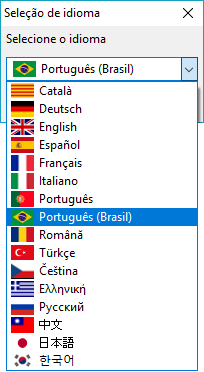
\includegraphics[scale=0.7]{invesalius_language_select_pt.png}
\end{figure}

\newpage

Enquanto o InVesalius é carregado, é exibida uma janela de abertura como a da figura
seguinte.

\begin{figure}[!htb]
\centering
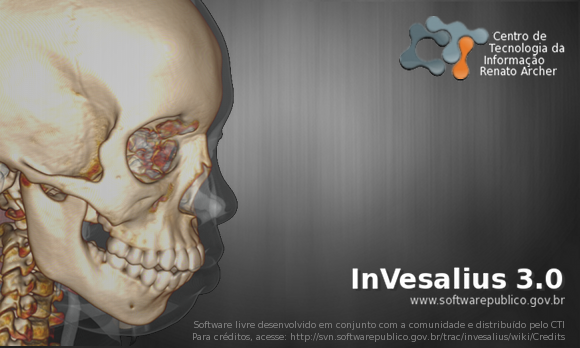
\includegraphics[scale=0.4]{splash_pt.png}
\end{figure}

\hspace{.2cm}

Em seguida, a janela principal do programa é aberta.

\begin{figure}[!htb]
\centering
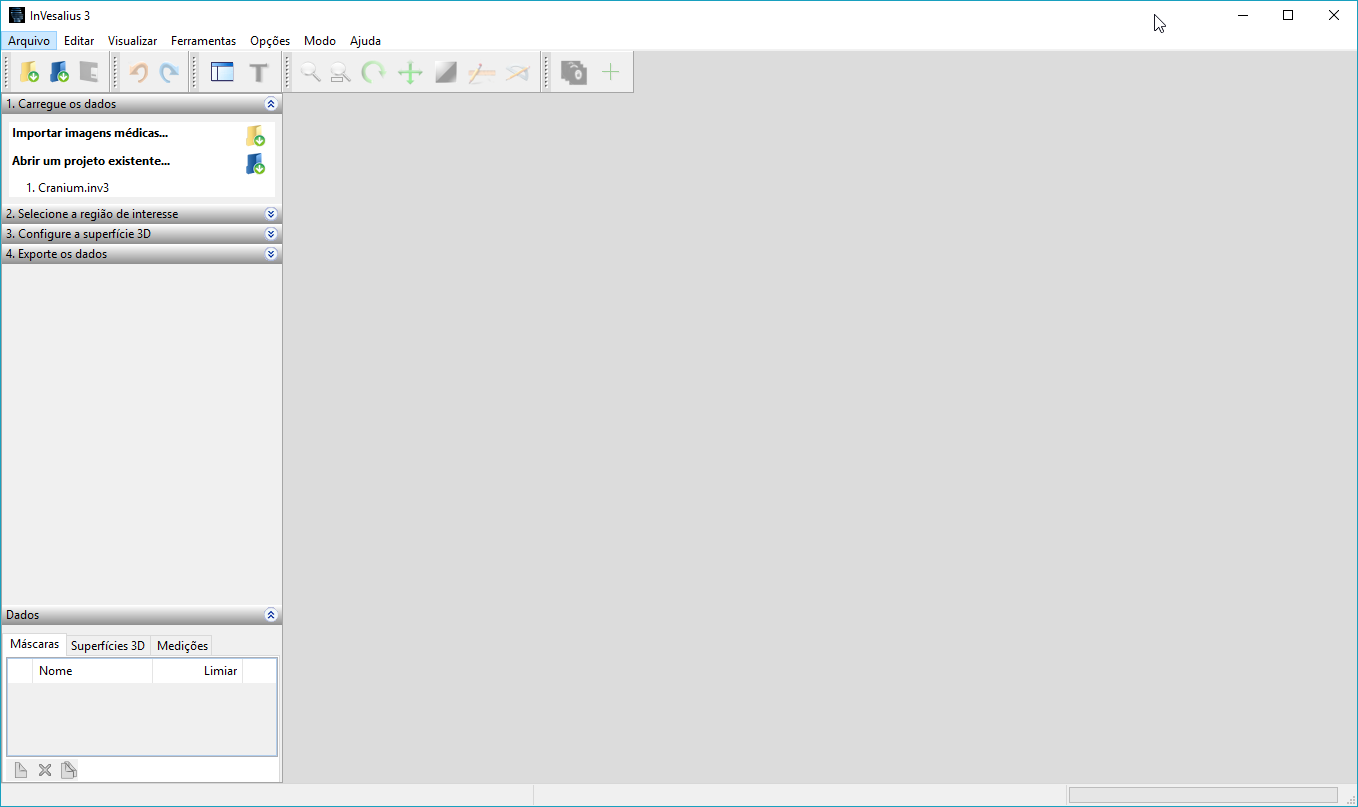
\includegraphics[scale=0.3]{main_window_without_project_pt.png}
\end{figure}

\section{Mac Os X}

Para iniciar a instalação no Mac Os X, clique 2 vezes com o botão esquerdo do mouse sobre o instalador.
Em seguida o instalador será inicializado.

\begin{figure}[!htb]
\centering
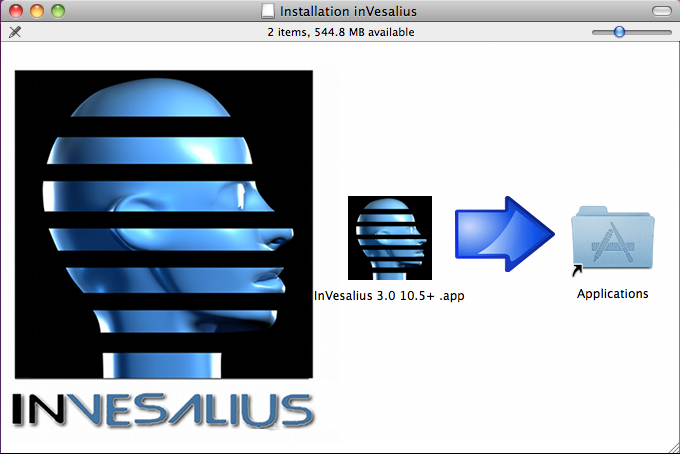
\includegraphics[scale=0.3]{mac2.png}
\end{figure}

Mantenha o botão esquerdo pressionado sobre o ícone do software InVesalius e arraste-o para o ícone \textit{Applications}
ambos contidos no instalador.

\begin{figure}[!htb]
\centering
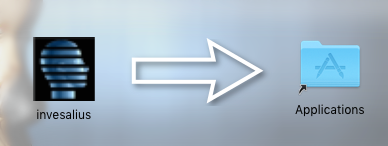
\includegraphics[scale=0.4]{mac4.png}
\end{figure}

O software já encontra-se instalado, bastando acessar pelo menu
